\chapter{OPIS ROZWIĄZANIA}
\label{chapter:opis_rozwiazania}

\section{Architektura systemu}

System składa się z pięciu głównych komponentów: nadajników BLE (ang. \textit{BLE beacon}), aplikacji mobilnej, systemu Wit.ai, serwera oraz bazy danych. Grafikę przedstawiającą architekturę systemu można zobaczyć na rysunku \ref{fig:architecture}.

\begin{figure}[H]
    \centering
    \includesvg[width=\textwidth]{images/architecture.svg}
    \caption{Architektura systemu.}
    \label{fig:architecture}
\end{figure}

Aplikacja mobilna jest odpowiedzialna za odbieranie oraz przetwarzanie sygnału z nadajników. Jej zadaniem jest również interakcja z użytkownikiem i wysyłanie zapytań do serwera. Serwer przetwarza żądania użytkownika, wysyła zapytania do API (ang. \textit{Application Programming Interface}) serwisu Wit.ai, oraz komunikuje się z bazą danych. Baza danych przechowuje dane i modyfikuje lub udostępnia je na żadanie serwera. Komunikacja między aplikacją mobilną a serwerem odbywa się za pomocą protokołu HTTP. Serwer jest odpowiedzialny za przetwarzanie żądań użytkownika, a także za komunikację z bazą danych. Baza danych przechowuje dane o produktach, użytkownikach, koszykach, sklepach itp.

\section{Baza danych}

\subsection{Opis bazy danych}

Baza danych została zaimplementowana w PostgreSQL. Wybór tej bazy danych wynika z jej wszechstronności, wydajności oraz możliwości łatwego skalowania. 

PostgreSQL to obiektowo-relacyjny system zarządzania bazami danych (ang. ORDBMS \textit{Object-Relational Database Management System}), którego rozwój rozpoczął się już w 1977 roku. Jego korzenie sięgają projektu o nazwie Ingres, realizowanego na Uniwersytecie Kalifornijskim w Berkeley.
Uznawany jest za jeden z najbardziej zaawansowanych systemów baz danych o otwartym kodzie źródłowym na świecie. Oferuje wiele funkcji, które do tej pory były kojarzone głównie z komercyjnymi rozwiązaniami klasy enterprise. \cite{worsley2002practical}

Baza danych przechowuje informacje o produktach, użytkownikach, koszykach oraz sklepach. Schemat bazy danych przedstawia rysunek \ref{fig:database}.

Struktura bazy danych została zaprojektowana w sposób modularny, umożliwiając efektywne zarządzanie danymi dotyczącymi sklepów, użytkowników oraz produktów. Główną tabelą bazy danych jest tabela \textit{stores}, która przechowuje informacje o sklepach, takie jak nazwa, współrzędne geograficzne oraz miasto. Związek tej tabeli z tabelą \textit{sections} umożliwia podział sklepów na sekcje, które z kolei są przypisane do tabeli \textit{categories}, zawierającej dane o kategoriach produktów.

Produkty są przechowywane w tabeli \textit{products}, gdzie każdy rekord zawiera szczegóły takie jak nazwa, opis, cena, dostępność, ilość oraz jednostka miary, przechowywana w tabeli \textit{units}. Relacje między tabelami \textit{categories} i \textit{p}roducts pozwalają na przypisanie każdego produktu do konkretnej kategorii, co ułatwia organizację i wyszukiwanie danych.

Użytkownicy systemu są reprezentowani w tabeli \textit{users}, gdzie zapisywane są ich dane personalne, takie jak imię, nazwisko, adres e-mail oraz zaszyfrowane hasło. Każdy użytkownik może posiadać wiele koszyków zakupowych, co jest odzwierciedlone w tabeli \textit{carts}, przechowującej informacje o koszykach, takie jak data utworzenia i powiązanie z użytkownikiem. 
Szczegóły dotyczące zawartości koszyków są zapisane w tabeli \textit{cart\_items}, która łączy produkty z koszykami i zawiera informacje o liczbie sztuk danego produktu.

Relacje pomiędzy tabelami są realizowane za pomocą kluczy obcych, z zastosowaniem reguły ON DELETE CASCADE, co zapewnia integralność danych oraz automatyczne usuwanie powiązanych rekordów w przypadku usunięcia danych z tabel nadrzędnych. Taka organizacja umożliwia łatwe skalowanie bazy danych oraz wspiera utrzymanie spójności danych w systemie.

\begin{figure}[H]
    \includesvg[width=\textwidth]{images/database.svg}
    \caption{Schemat bazy danych.}
    \label{fig:database}
\end{figure}

\subsection{Szczegółowy opis tabel}

\subsubsection{Tabela stores}
\begin{itemize}
\item store\_id - SERIAL PRIMARY KEY: Unikalny identyfikator każdego sklepu.
\item store\_name - VARCHAR(255) NOT NULL: Nazwa sklepu.
\item latitude - VARCHAR(255) NOT NULL: Szerokość geograficzna określająca położenie sklepu.
\item longitude - VARCHAR(255) NOT NULL: Długość geograficzna określająca położenie sklepu.
\item city - VARCHAR(255) NOT NULL: Miasto, w którym znajduje się sklep.
\end{itemize}

\subsubsection{Tabela sections}
\begin{itemize}
\item section\_id - SERIAL PRIMARY KEY: Unikalny identyfikator sekcji sklepu.
\item section\_name - VARCHAR(255) NOT NULL: Nazwa sekcji w sklepie.
\item store\_id - INT REFERENCES stores(store\_id) ON DELETE CASCADE: Klucz obcy wskazujący sklep, do którego należy sekcja.
\end{itemize}

\subsubsection{Tabela categories}
\begin{itemize}
\item category\_id - SERIAL PRIMARY KEY: Unikalny identyfikator kategorii.
\item category\_name - VARCHAR(255) NOT NULL: Nazwa kategorii produktów.
\item section\_id - INT REFERENCES sections(section\_id) ON DELETE CASCADE: Klucz obcy wskazujący sekcję, do której przypisana jest kategoria.
\end{itemize}

\subsubsection{Tabela units}
\begin{itemize}
\item unit\_id - SERIAL PRIMARY KEY: Unikalny identyfikator jednostki miary.
\item unit\_name - VARCHAR(50) NOT NULL: Pełna nazwa jednostki miary (np. “kilogram”).
\item unit\_symbol - VARCHAR(10) NOT NULL: Skrót jednostki miary (np. “kg”).
\end{itemize}

\subsubsection{Tabela products}
\begin{itemize}
\item product\_id - SERIAL PRIMARY KEY: Unikalny identyfikator produktu.
\item name - VARCHAR(255) NOT NULL: Nazwa produktu.
\item description - TEXT: Opis produktu.
\item price - DECIMAL(10,2) NOT NULL: Cena produktu w formacie dziesiętnym (np. 123.45).
\item category\_id - INT REFERENCES categories(category\_id) ON DELETE CASCADE: Klucz obcy wskazujący kategorię, do której należy produkt.
\item availability - VARCHAR(50) NOT NULL: Status dostępności produktu (np. “w magazynie”).
\item amount - DECIMAL(10,2) NOT NULL: Ilość dostępna w magazynie.
\item unit\_id - INT REFERENCES units(unit\_id) ON DELETE CASCADE: Klucz obcy wskazujący jednostkę miary produktu.
\end{itemize}

\subsubsection{Tabela users}
\begin{itemize}
\item user\_id - SERIAL PRIMARY KEY: Unikalny identyfikator użytkownika.
\item email - VARCHAR(255) UNIQUE NOT NULL: Adres e-mail użytkownika.
\item password - VARCHAR(255) NOT NULL: Hasło użytkownika (w formie zaszyfrowanej).
\item first\_name - VARCHAR(50) NOT NULL: Imię użytkownika.
\item last\_name - VARCHAR(50) NOT NULL: Nazwisko użytkownika.
\end{itemize}

\subsubsection{Tabela carts}
\begin{itemize}
\item cart\_id - SERIAL PRIMARY KEY: Unikalny identyfikator koszyka.
\item user\_id - INT REFERENCES users(user\_id) ON DELETE CASCADE: Klucz obcy wskazujący użytkownika, do którego należy koszyk.
\item creation\_date - TIMESTAMP DEFAULT CURRENT\_TIMESTAMP: Data i czas utworzenia koszyka.
\end{itemize}

\subsubsection{Tabela cart\_items}
\begin{itemize}
\item cart\_item\_id - SERIAL PRIMARY KEY: Unikalny identyfikator pozycji w koszyku.
\item cart\_id - INT REFERENCES carts(cart\_id) ON DELETE CASCADE: Klucz obcy wskazujący koszyk, do którego należy pozycja.
\item product\_id - INT REFERENCES products(product\_id) ON DELETE CASCADE: Klucz obcy wskazujący produkt dodany do koszyka.
\item quantity - INT NOT NULL: Liczba sztuk danego produktu w koszyku.
\end{itemize}

tekst

\section{Interfejs użytkownika}

\subsection{Opis dostępnych widoków}

\subsubsection{Strona tytułowa}

Strona tytułowa aplikacji pełni funkcję ekranu startowego, witając odbiorcę logiem oraz hasłem zachęcającym do korzystania z aplikacji. Widnieje na niej przycisk \textit{Get Started}, który umożliwia przejście do kolejnych widoków. Jeśli eksploatator był zalogowany w ciągu ostatnich 7 dni, aplikacja przekierowuje go do widoku logowania. W przeciwnym wypadku trafia on do ekranu profilu. 

\begin{center} 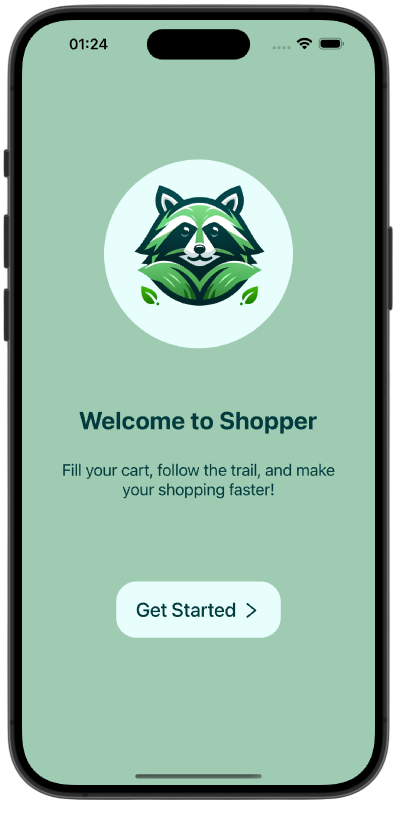
\includegraphics[width=0.3\textwidth]{images/front/home_page.png} \end{center}


Całość utrzymana jest w przyjaznej stylistyce, z dominującym odcieniem zieleni oraz spójną paletą kolorów, wygenerowaną przez narzędzie DALL·E 3 od OpenAI.

\begin{center} 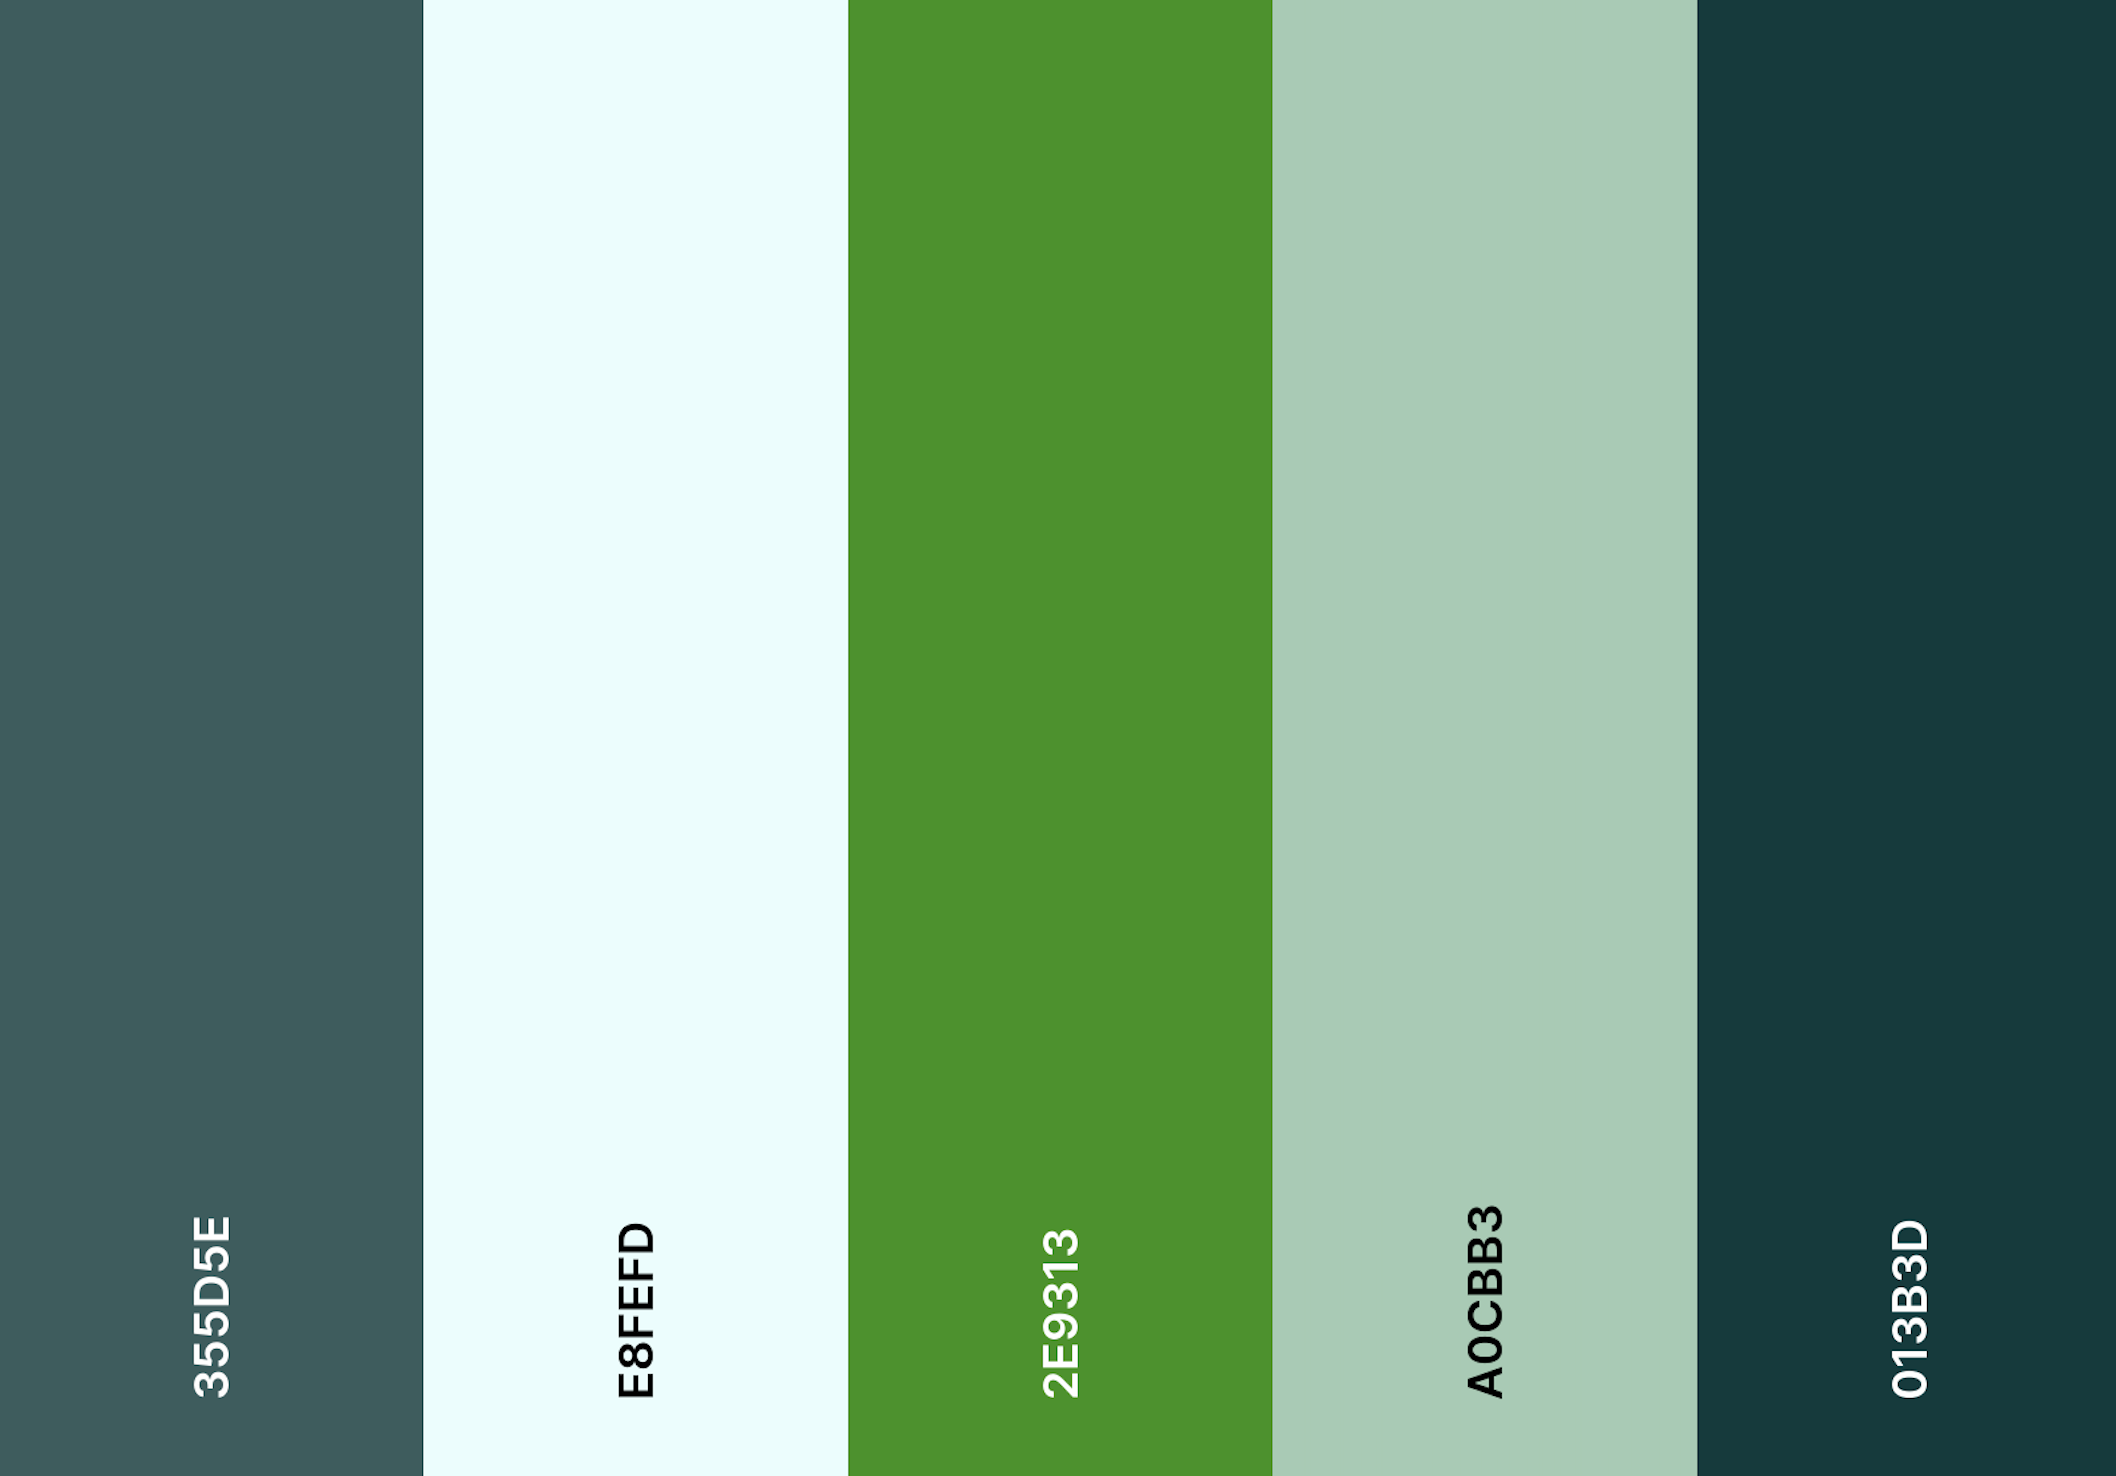
\includegraphics[width=0.3\textwidth]{images/front/theme.png} \end{center}

\subsubsection{Ekran logowania}

Ekran logowania umożliwia odbiorcy uwierzytelnienie w aplikacji, poprzez wprowadzenie adresu e-mail oraz hasła. Jego głównym celem jest weryfikacja tożsamości eksploatatora oraz przekierowanie do dalszych widoków w zależności od wyniku logowania. 

\begin{center} 
    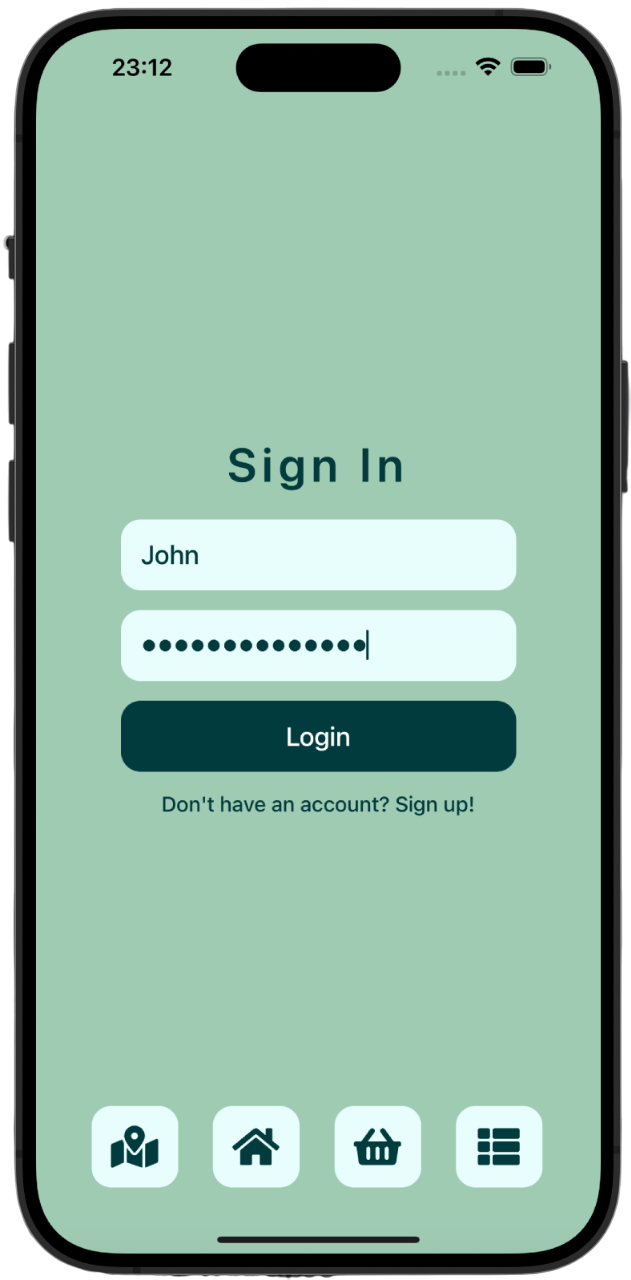
\includegraphics[width=0.3\textwidth]{images/front/login_page.png} 
\end{center}

Górną część widoku stanowi nagłówek \textit{Sign In}, który podkreśla cel ekranu. Tuż pod nim znajduje się formularz składający się z dwóch pól tekstowych: jednego przeznaczonego do wprowadzania adresu e-mail, a drugiego do hasła, z cechą ukrywania wprowadzanych znaków. Naciśnięcie przycisku \textit{Login} uruchamia logikę, która weryfikuje tożsamość odbiorcy na podstawie danych wprowadzonych w polach tekstowych. W przypadku niepowodzenia gość otrzymuje odpowiedni komunikat, informujący o niepoprawnym e-mailu lub haśle. Dla nowych kupujących, widok zapewnia przejście do ekranu rejestracji, poprzez kliknięcie w link \textit{Don't have an account? Sign up!}. 

Dolną część ekranu zajmuje pasek nawigacyjny z ikonami, które przenoszą do kolejnych podstron: mapy sklepów, profilu odbiorcy, kategorii produktów wybranego sklepu oraz strony tytułowej. Tylko ta ostatnia jest dostępna dla niezalogowanych użytkowników.

\begin{center} 
    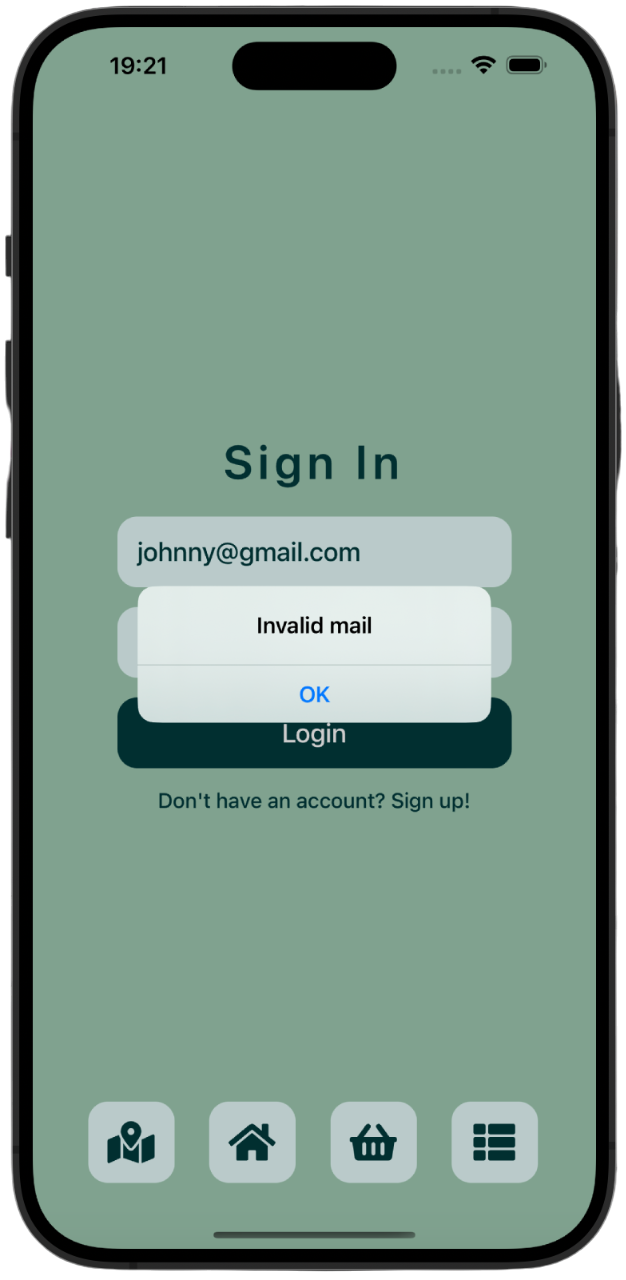
\includegraphics[width=0.3\textwidth]{images/front/login_invalid.png} 
    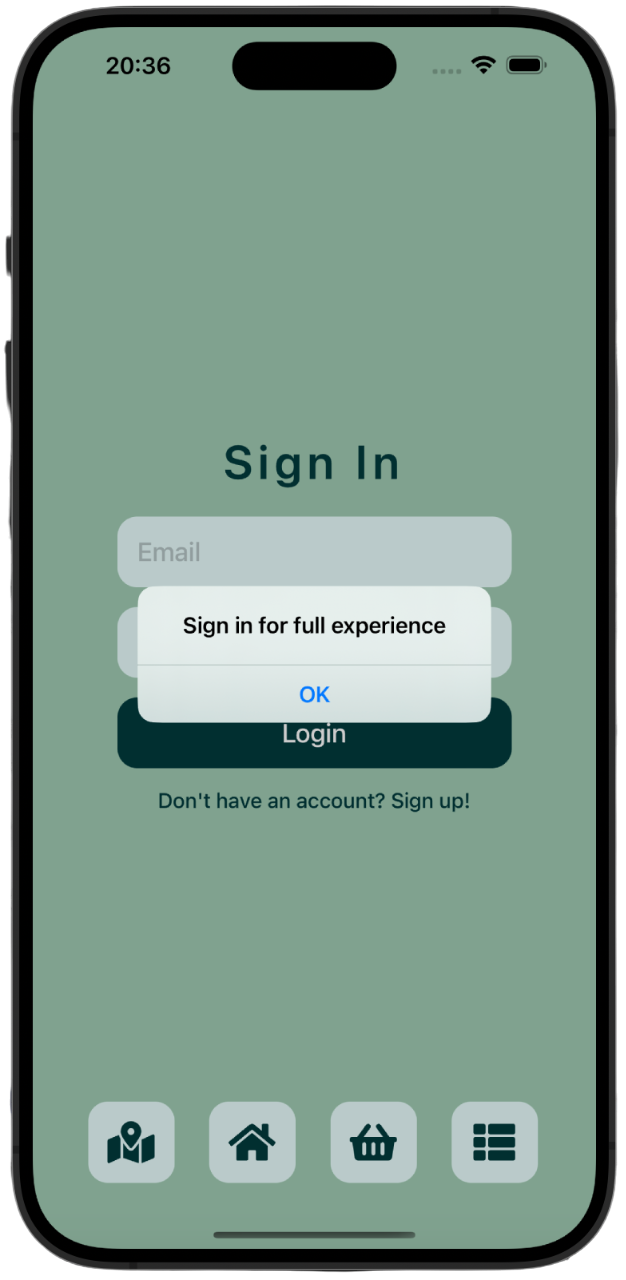
\includegraphics[width=0.3\textwidth]{images/front/login_not_signed.png} 
\end{center}

\subsubsection{Rejestracja użytkownika}

Ekran rejestracji umożliwia nowym odbiorcom założenie konta, co jest niezbędne do korzystania z funkcji wymagających uwierzytelnienia, takich jak dodawanie produktów do koszyka czy przeglądanie sklepów na mapie. Formularz rejestracyjny składa się z kilku pól:
\begin{itemize} \item \textit{Firstname} i \textit{Lastname} – wymagane minimum trzech znaków, by dane były wystarczająco szczegółowe. \item \textit{Email} – odbiorca podaje swój adres e-mail, który jest weryfikowany pod kątem poprawności formatu (obecność znaku \textit{@} oraz domeny). \item \textit{Password} i \textit{Repeat password} – hasło musi mieć co najmniej osiem znaków i być identyczne w obu polach. Dodatkowo, tekst wprowadzony w tych polach jest ukrywany, aby zapewnić prywatność. \end{itemize}

\begin{center} 
    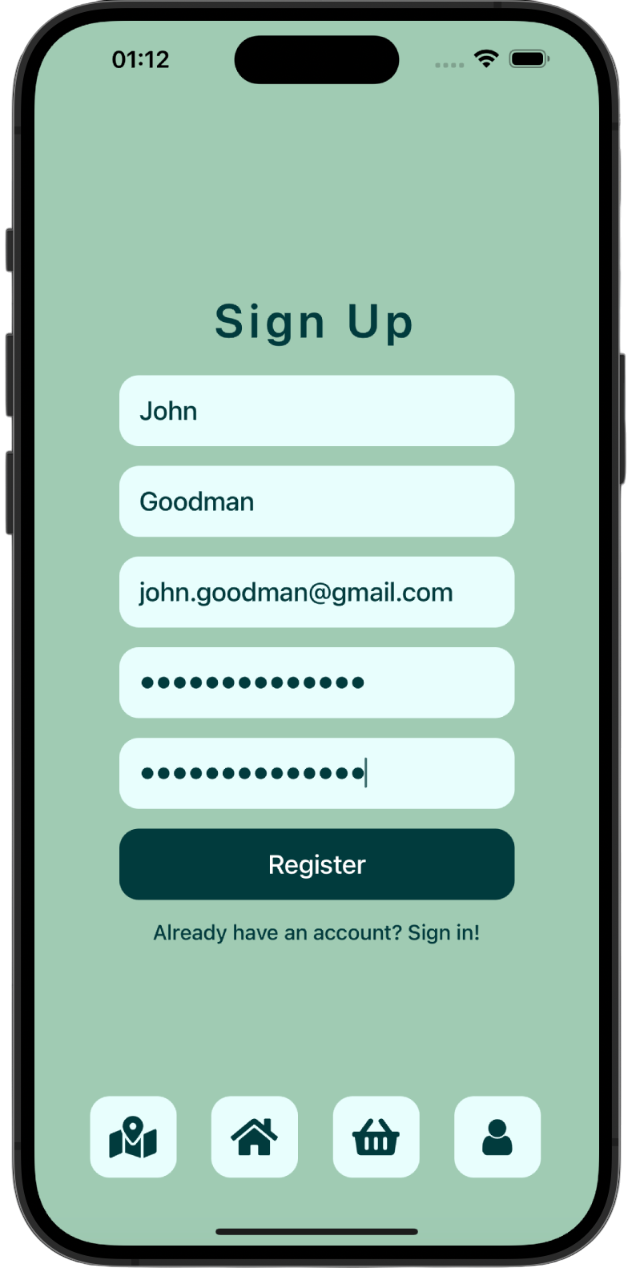
\includegraphics[width=0.3\textwidth]{images/front/register_page.png}
\end{center}

Po wypełnieniu formularza, należy wcisnąć guzik \textit{Register}, po którym odbywa się walidacja danych. W przypadku spełnienia warunków wpisanych pól, nowy użytkownik, wraz z koszykiem jest rejestrowany w bazie danych. Po zakończeniu rejestracji następuje automatyczne zalogowanie, a imię oraz ID są zapisywane w lokalnej pamięci urządzenia, w bezpieczny sposób, aby dane nie trafiły w niepowołane ręce. Pozwala to na sprawne obslużenie mechanizmu sesji oraz dostępu do koszyka jego właściciela. Następuje po tym przekierowanie do ekranu kategorii produktów wybranego sklepu. Jeśli dane są nieprawidłowe, wyświetlane są stosowne komunikaty, informujące o błędach, takich jak niewłaściwy format e-maila, zbyt krótkie hasło czy jego niezgodność. Osoby posiadające już konto mogą skorzystać z linku \textit{Already have an account? Sign in!}, znajdującego się pod formularzem, aby przejść do ekranu logowania. 

Dolną część ekranu zajmuje pasek nawigacyjny, który zawiera przyciski prowadzące do kolejnych sekcji aplikacji. Pierwszy z nich przekierowuje do widoku mapy sklepów. Kolejny przekierowuje na stronę główną – jest to jedyny dostępny dla niezalogowanych odbiorców. Trzeci zawiera ikonę koszyka, w którym użytkownicy mogą przeglądać swoje produkty, a czwarty prowadzi do profilu odbiorcy, gdzie można zarządzać danymi konta.

\begin{center} 
    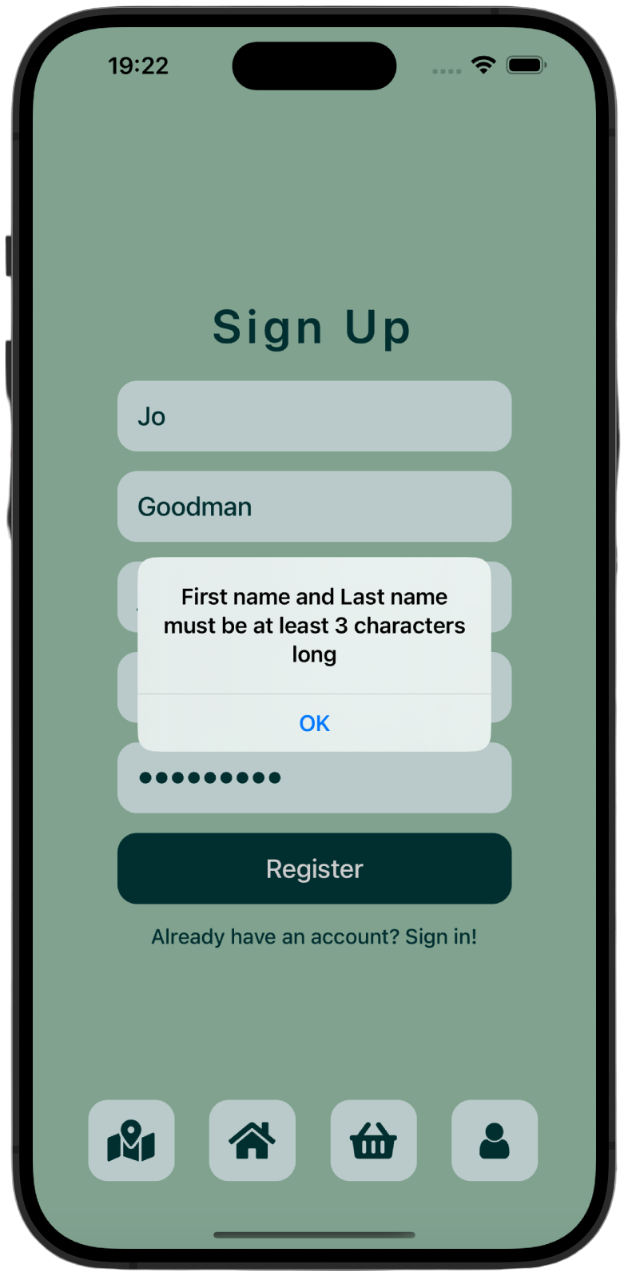
\includegraphics[width=0.3\textwidth]{images/front/register_invalid.png}
\end{center}

\subsubsection{Kategorie produktów}

Ekran kategorii stanowi pierwszy krok do przeglądania dostępnych produktów w wybranym sklepie. Centralnym elementem tego widoku jest siatka kategorii, umożliwiająca użytkownikowi intuicyjne poruszanie się po różnych grupach produktów. 

\begin{center} 
    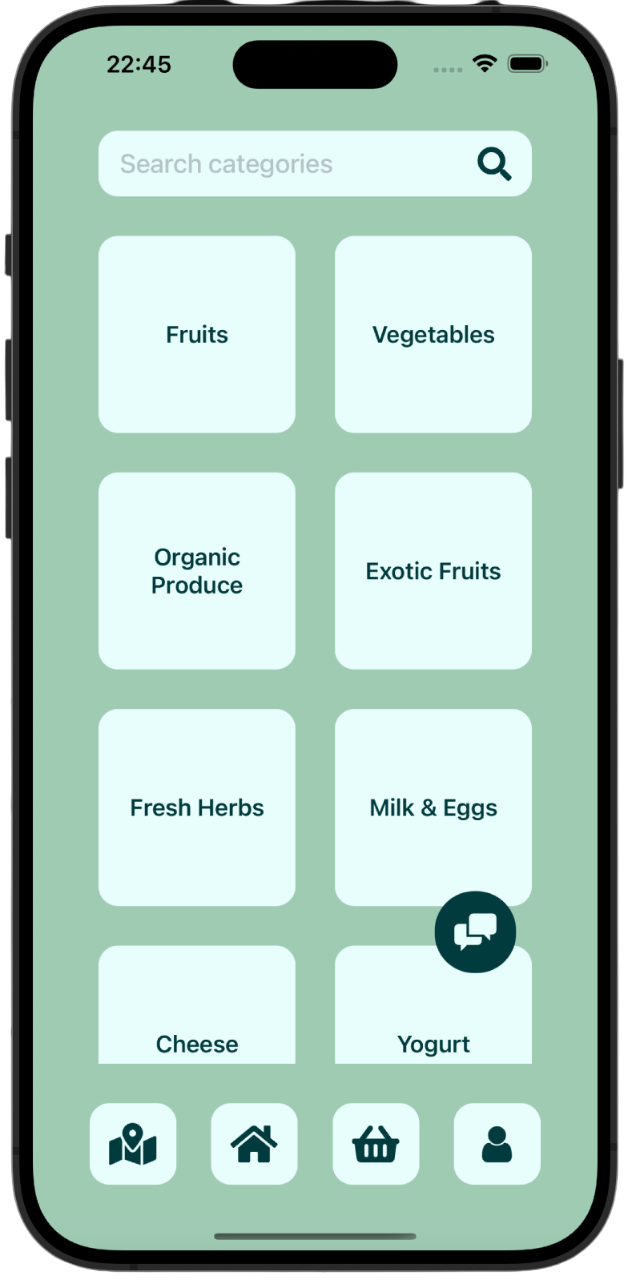
\includegraphics[width=0.3\textwidth]{images/front/categories_page.png} 
\end{center}

W górnej części widoku znajduje się pasek wyszukiwania, składający się z pola tekstowego oraz ikony lupy, umożliwiający szybkie filtrowanie kategorii na podstawie wprowadzonego tekstu. Wprowadzenie frazy w pole wyszukiwania automatycznie ogranicza widoczne wyniki, wyświetlając jedynie pasujące grupy produktów. Każdy kafelek siatki zawiera nazwę kategorii, a jego kliknięcie przekierowuje użytkownika do widoku produktów należących do wybranej kategorii. Siatkę można przewijać w pionie, aby odkrywać kolejne kafelki dostępne z listy. 

Dolną część ekranu zajmuje pasek nawigacyjny, który umożliwia szybki dostęp do innych kluczowych widoków aplikacji, takich jak mapa sklepów, profil użytkownika, koszyk oraz strona tytułowa. Widok zawiera również przeciągany dymek czatu, który pozwala na szybki kontakt z obsługą klienta. Jest on towarzyszem większości ekranów aplikacji, przez co został mu poświęcony osobny artykuł w sekcji o numerze \textit{x.x.x}.

\begin{center} 
    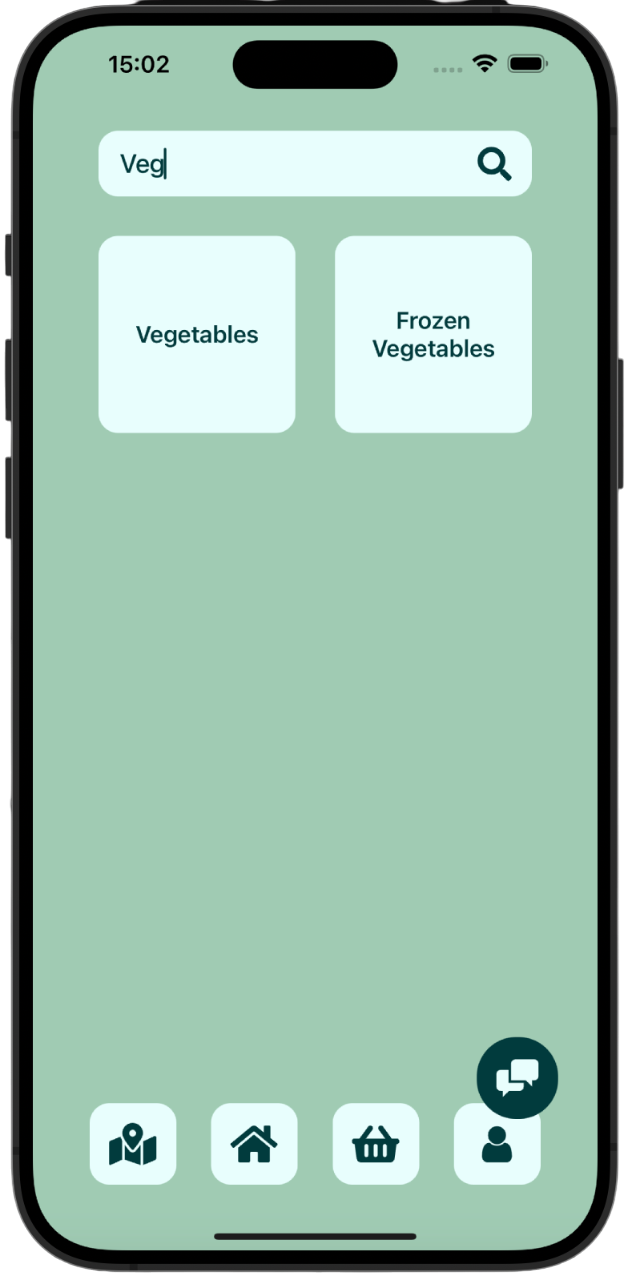
\includegraphics[width=0.3\textwidth]{images/front/categories_filtered.png} 
\end{center}

\subsubsection{Ekran produktów}

Ekran produktów pozwala użytkownikowi na przeglądanie i dodawanie do koszyka artykułów należących do wybranej kategorii. 

\begin{center} 
    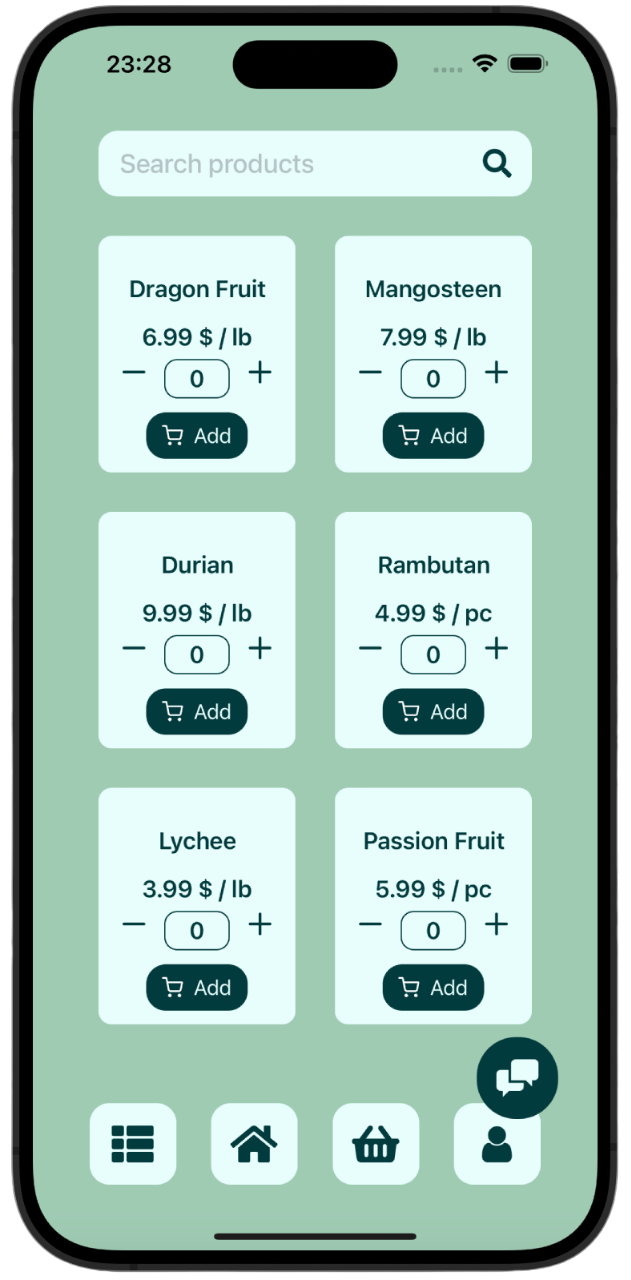
\includegraphics[width=0.3\textwidth]{images/front/products_page.png}  
\end{center}

Na samej górze widoku znajduje się pasek wyszukiwania, umożliwiający szybkie filtrowanie produktów po ich nazwie. Pasek zawiera pole tekstowe oraz ikonę lupy. Wprowadzenie tekstu w tym polu automatycznie zawęża widok, prezentując jedynie pasujące wyniki. Poniżej znajduje się przewijalna siatka produktów, w której każdy kafelek zawiera nazwę produktu, cenę oraz symbol jednostki miary. Dodatkowo dla każdego produktu dostępne są przyciski \textit{+} i \textit{–}, umożliwiające zwiększanie lub zmniejszanie ilości produktu, jaką użytkownik chce dodać do koszyka. Wartość wprowadzana przez kupującego jest automatycznie walidowana. Walidacja polega na sprawdzeniu, czy wprowadzony symbol jest liczbą całkowitą. Wartości mniejsze od zera nie są akceptowane. Pod każdym kafelkiem produktu znajduje się przycisk \textit{Add}, który dodaje wybraną ilość artykułu do koszyka gościa. Po naciśnięciu przycisku aplikacja odpowiednio weryfikuje możliwość dokonania zakupu poprzez sprawdzenie ilości produktu w magazynie. W przypadku błędnych danych, takich jak ilość większa niż dostępna, użytkownik otrzymuje odpowiedni komunikat w postaci alertu. 

Dół ekranu zdobi pasek nawigacyjny, który umożliwia powrót do ekranu kategorii, sprawdzenie stanu koszyka, przejście do profilu użytkownika czy strony głównej.

\begin{center} 
    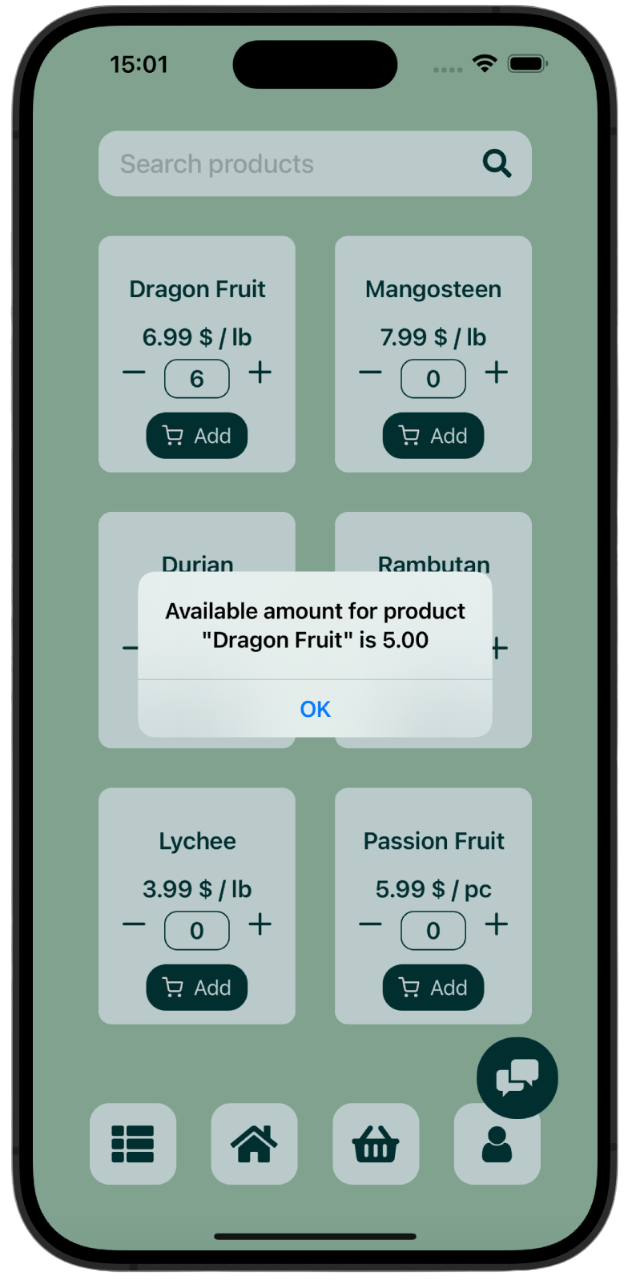
\includegraphics[width=0.3\textwidth]{images/front/products_amount.png}  
    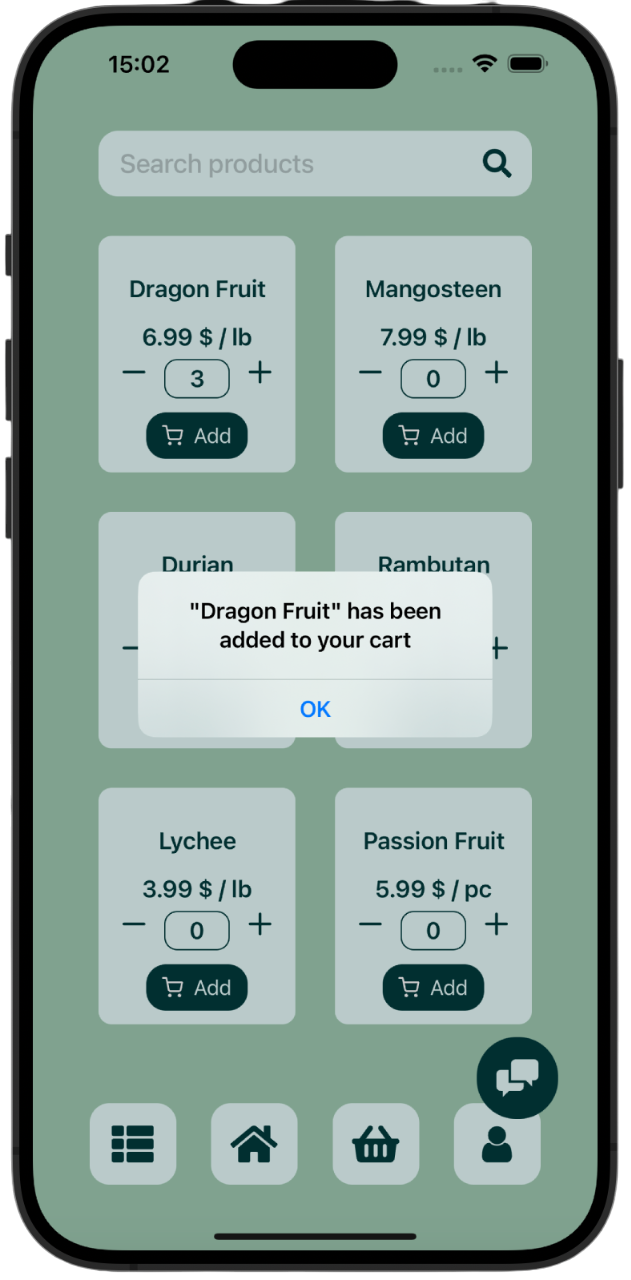
\includegraphics[width=0.3\textwidth]{images/front/products_added.png}  
\end{center}

\subsubsection{Koszyk użytkownika}

Ekran koszyka pozwala użytkownikowi zarządzać produktami dodanymi do koszyka oraz przygotować się do finalizacji zakupów. 

\begin{center}
    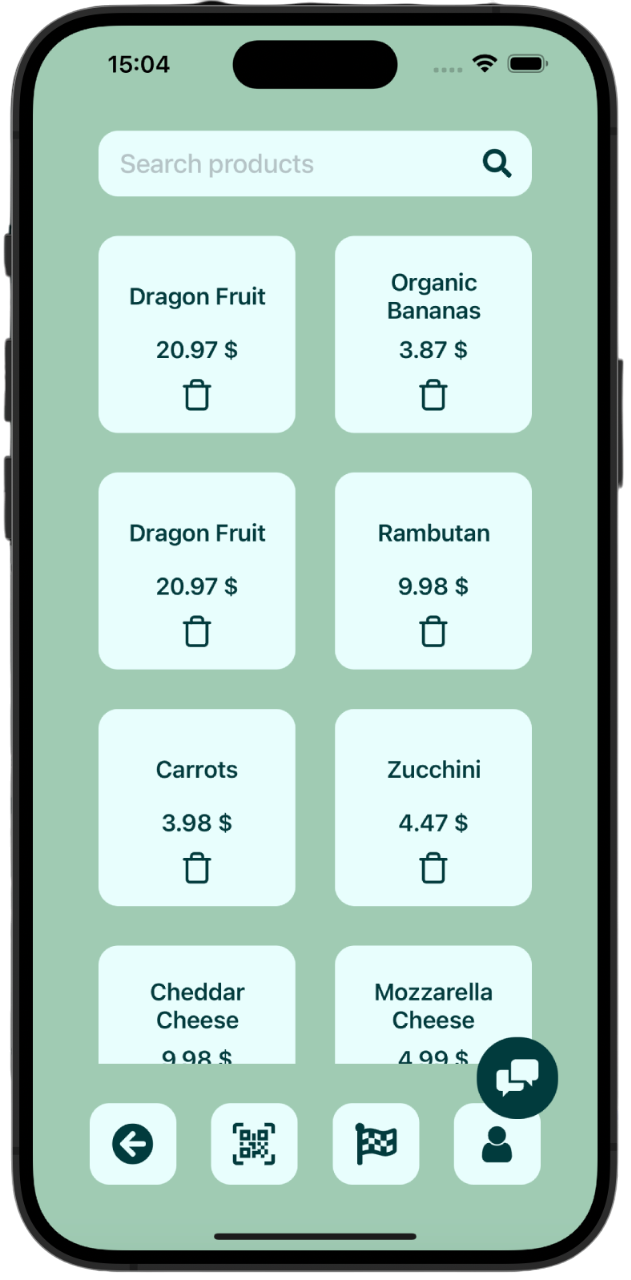
\includegraphics[width=0.3\textwidth]{images/front/cart_page.png}
\end{center}

W górnej części ekranu znajduje się pasek wyszukiwania, umożliwiający filtrowanie produktów według nazwy. Użytkownik może wprowadzić frazę w polu tekstowym, aby zawęzić listę wyświetlanych produktów, co znacznie ułatwia nawigację w przypadku dużej liczby elementów. Listę produktów w koszyku prezentuje przewijalna siatka, mieszcząca się pod paskiem wyszukiwania. Każdy element listy produktów w koszyku zawiera następujące informacje:
\begin{itemize}
    \item Nazwę produktu.
    \item Cenę jednostkową.
    \item Ilość produktu w koszyku, wyrażoną w odpowiedniej jednostce miary (np. sztuki, kilogramy).
    \item Łączną cenę dla danej pozycji, obliczoną jako iloczyn ceny jednostkowej i ilości.
\end{itemize}

W przypadku chęci usunięcia produktu z koszyka, użytkownik posiada możliwość kliknięcia na ikonkę kosza na śmieci danego produktu. Aplikacja automatycznie aktualizuje widok koszyka po każdej zmianie.

Dolną część ekranu zajmuje pasek nawigacyjny, który umożliwia szybkie przejście do kolejnych widoków aplikacji. Należą do nich: generowanie kodu qr, mapa nawigująca po sklepie, profil użytkownika oraz powrót do poprzedniego ekranu.

\begin{center}
    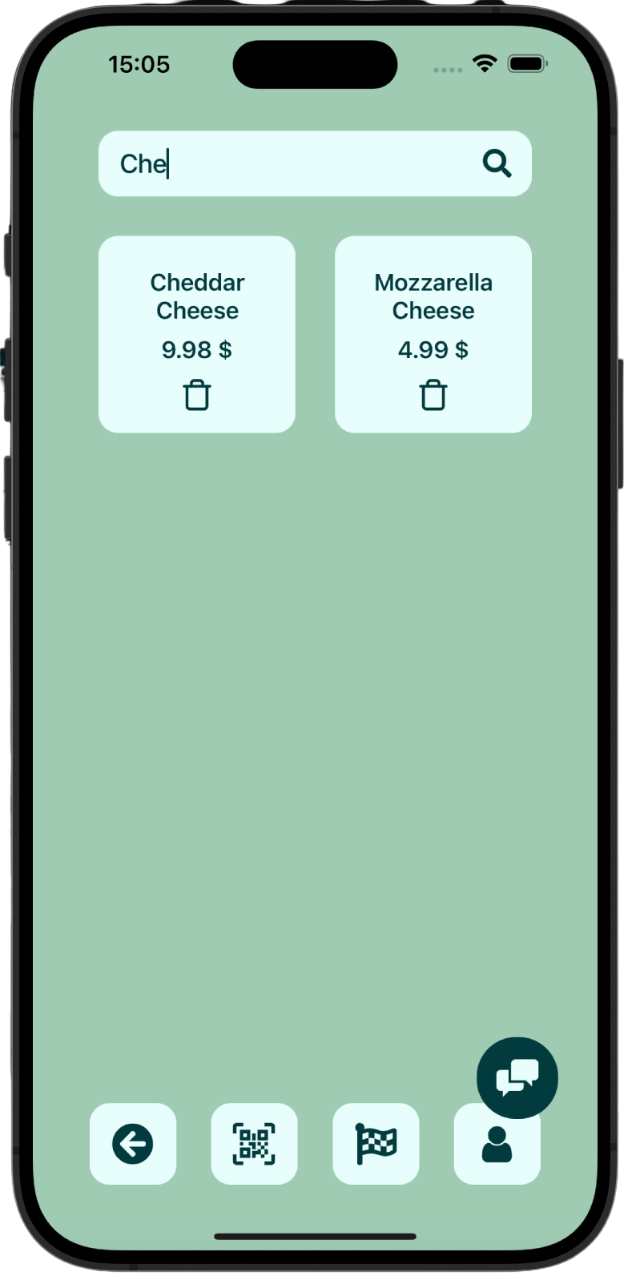
\includegraphics[width=0.3\textwidth]{images/front/cart_filtered.png}
\end{center}


\subsubsection{Generowanie kodu qr}

Po przejściu na ten ekran, pobierana jest lista produktów z koszyka danego kupującego. Dane na temat produktów zostają zawarte w wygenerowanym kodzie, który wyświetla się na środku ekranu po załadowaniu listy. W przypadku, gdy koszyk jest pusty, wyświetlany jest komunikat zachęcający do jego uzupełnienia. 

\begin{center}
    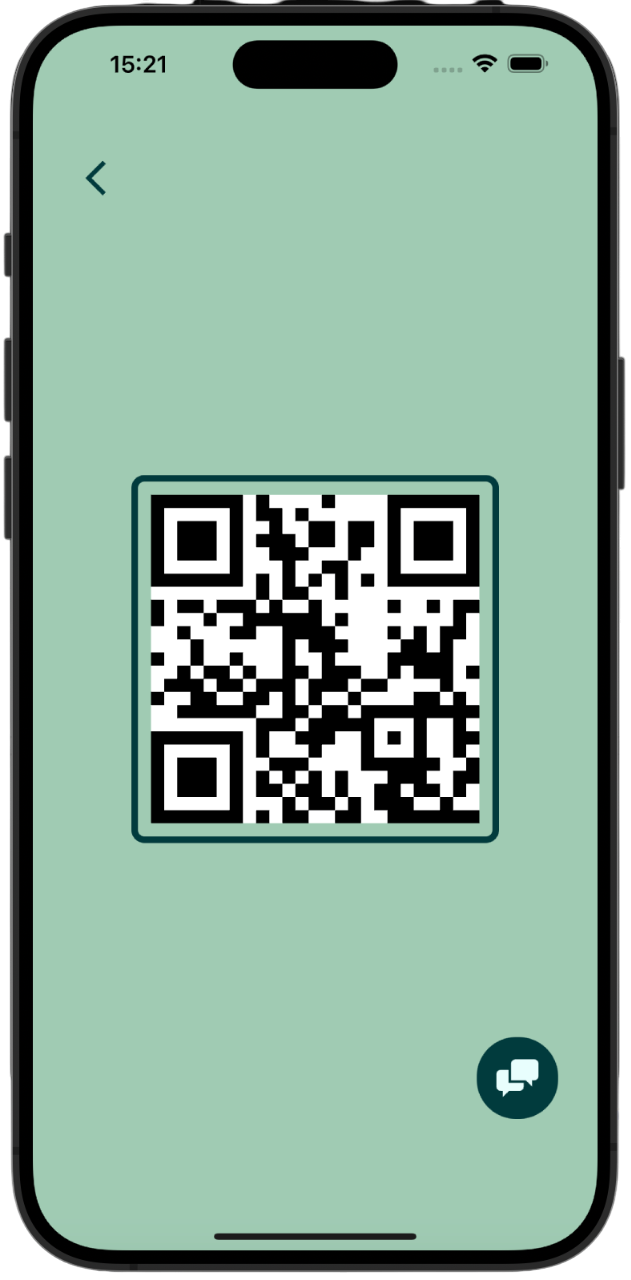
\includegraphics[width=0.3\textwidth]{images/front/qr_page.png}
\end{center}

Użytkownik ma możliwość zeskanowania kodu qr za pomocą czytnika danego sklepu, co pozwala na szybkie zinterowanie danych z aplikacją kasy samoobsługowej i nabicia zakupów na paragon. Za integrację kodu ze swoją aplikacją odpowiedzialny jest sam sklep. 

Aby wyjść z ekranu, należy nacisnąć symbol ptaszka, który przenosi użytkownika z powrotem do ekranu produktów.

\begin{center}
    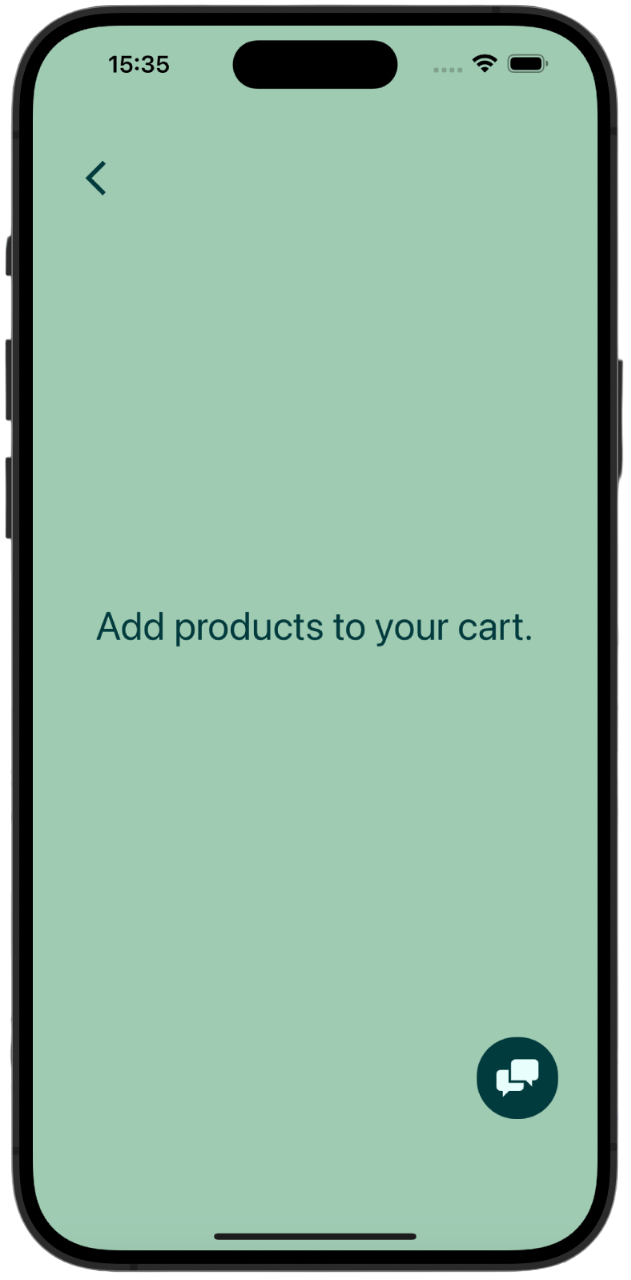
\includegraphics[width=0.3\textwidth]{images/front/qr_empty.png}
\end{center}

\subsubsection{Mapa sklepów}

Ekran wyboru sklepu pozwala użytkownikowi w intuicyjny sposób wybrać lokalizację sklepu, w którym planuje zrobić zakupy. Głównym elementem, pokrywającym cały widok jest interaktywna mapa, na której zaznaczone są wszystkie dostępne sklepy w formie markerów. Użytkownik może dowolnie przesuwać mapę oraz przybliżać i oddalać widok, aby lepiej zapoznać się z rozmieszczeniem sklepów. 

\begin{center}
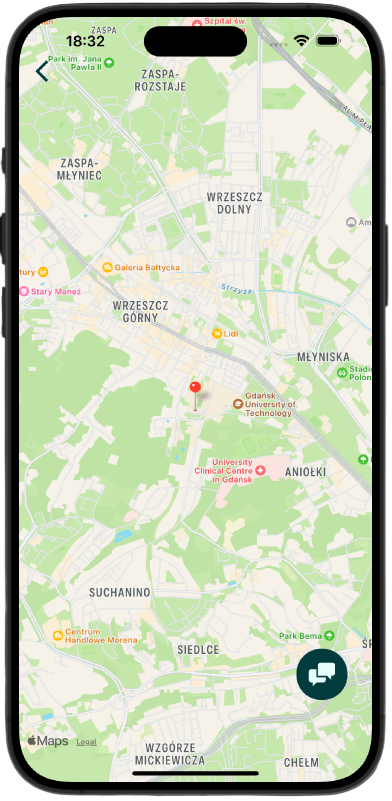
\includegraphics[width=0.3\textwidth]{images/front/store_page.png}
\end{center}

Punkt początkowy został ustawiony na sklep \textit{ETI PG} na potrzebę prezentacji. Kliknięcie na marker sklepu wyświetla szczegóły wybranej lokalizacji w dolnym panelu ekranu. Panel ten prezentuje nazwę sklepu oraz przycisk \textit{Select store}, który pozwala na potwierdzenie wyboru. Wybór sklepu jest sygnalizowany wyświetleniem komunikatu informującego o poprawnym zapisaniu decyzji. Dzięki temu użytkownik ma pewność, że jego wybór został zarejestrowany i aplikacja poprawnie zapisała ID sklepu, z którego należy pobrać kategorie i produkty.

W górnym lewym rogu ekranu znajduje się przycisk powrotu, który umożliwia szybkie przejście do poprzedniego widoku. 

\begin{center}
    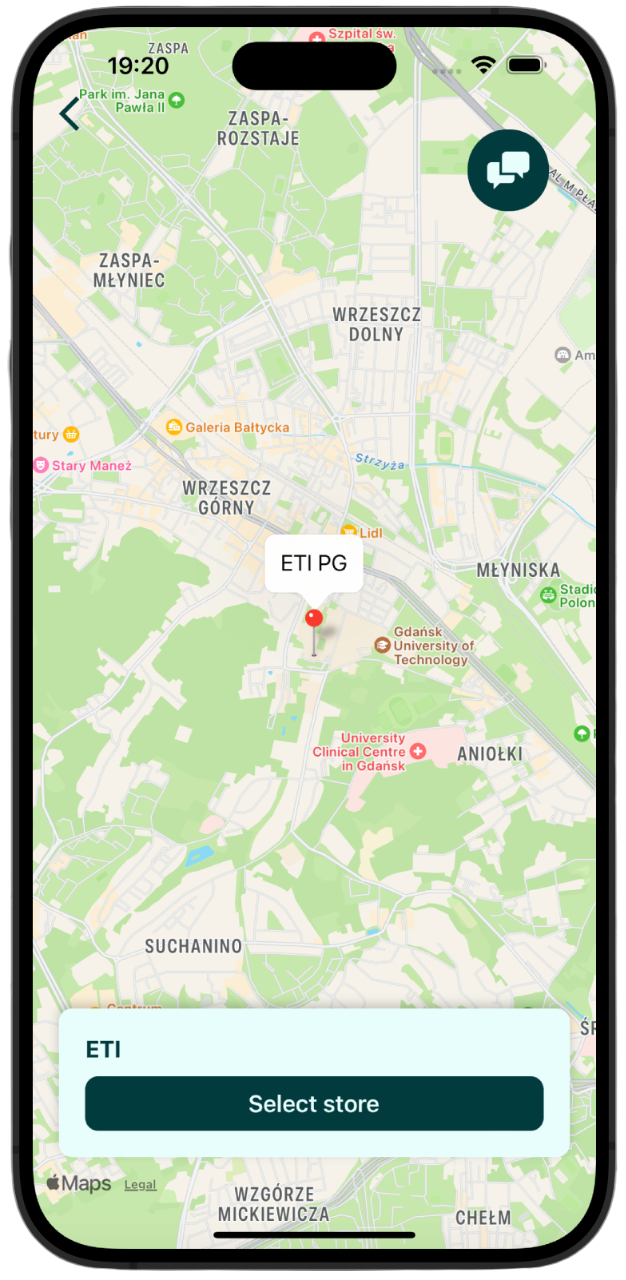
\includegraphics[width=0.3\textwidth]{images/front/store_selected.png}
    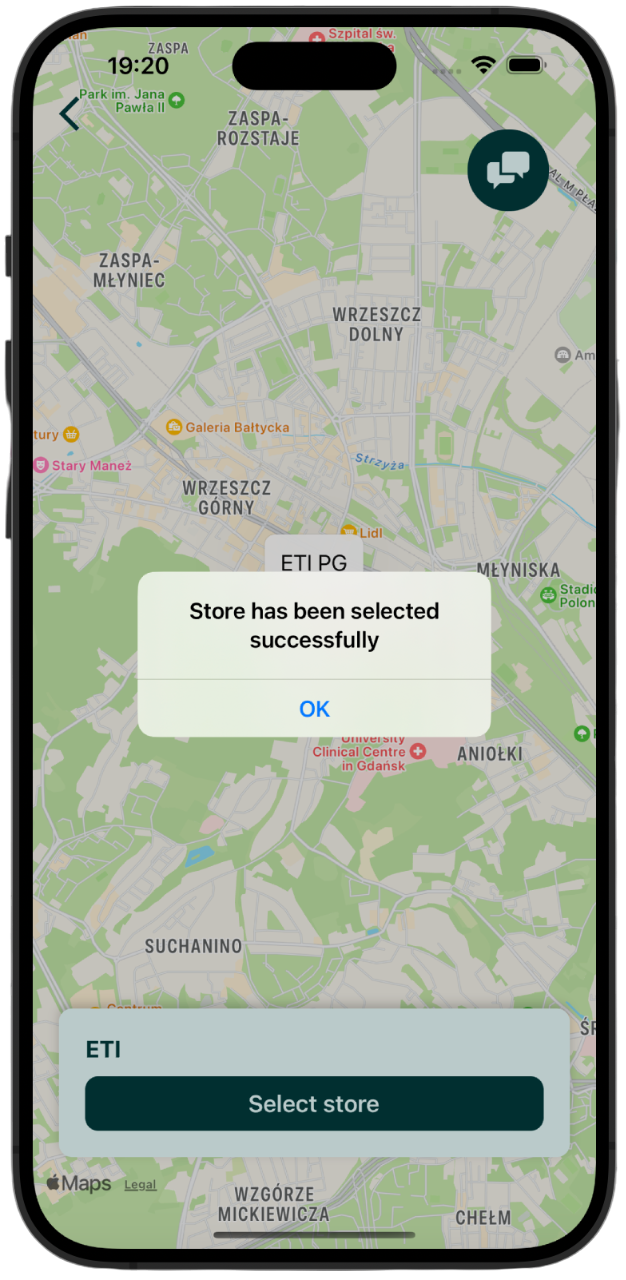
\includegraphics[width=0.3\textwidth]{images/front/store_success.png}
\end{center}


\subsubsection{Ekran nawigacji}

Ekran ten pozwala użytkownikowi na łatwe nawigowanie po sklepie, w celu zrealizowania zakupów w jak najkrótszym czasie. Jest to kluczowy widok, który odpowiada za podświetlenie klientowi trasy, jaką należy pokonać, aby uzyskać ten efekt.

\begin{center}
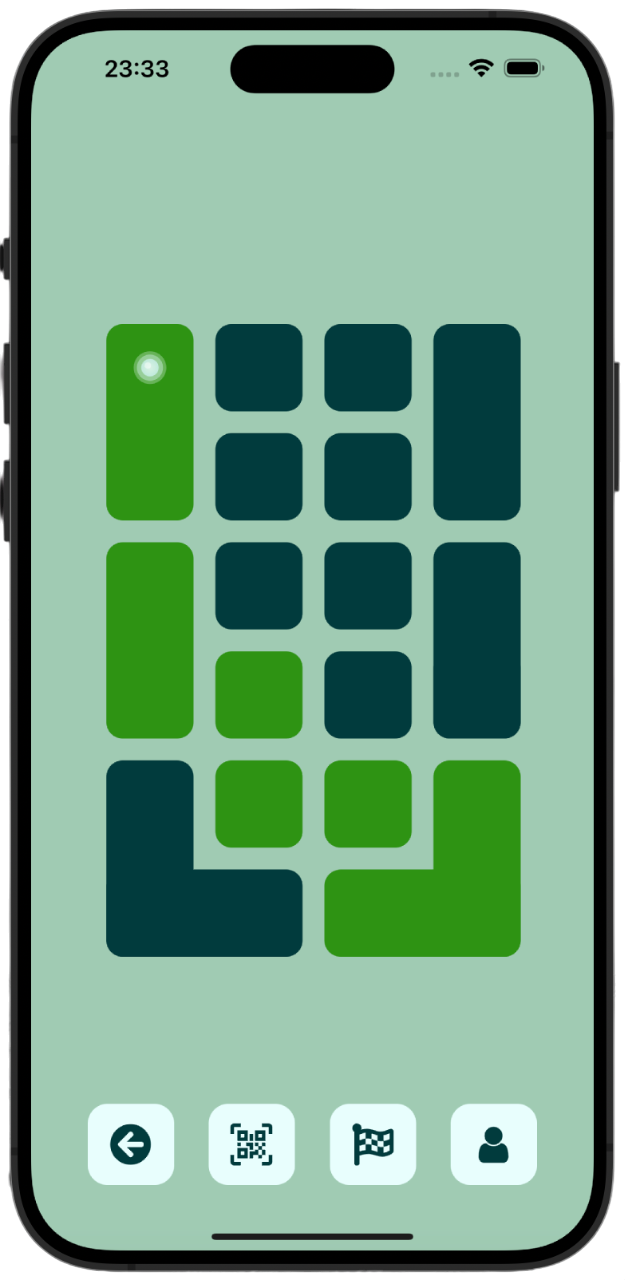
\includegraphics[width=0.3\textwidth]{images/front/navigation_page.png}
\end{center}

Ekran w znacznej większości składa się mapy sklepu, wygenerowanej ręcznie za pomocą grafiki SVG. Grafika ta, jest tworzona po wcześniejszej konsultacji ze sklepem. Podczas wejścia na ekran, aplikacja pobiera listę produktów z koszyka i na jej podstawie, wyznacza najkrótszą trasę, w postaci sektorów, które należy przebyć. Kolor trasy zmienia się na zielony, podczas gdy reszta sekcji pozostaje morska. Następnie za pomocą rozmieszczonych nadajników BLE, zostaje określone położenie użytkownika, które jest aktulizowane w czasie rzeczywistym, w postaci pulsującej, białej kropki.

Nawigacja w każdej chwili może zostać przerwana, chociażby poprzez powrót do koszyka, aby dodać kolejne produkty. W takim przypadku, po powrocie na ekran nawigacji, kupujący widzi nowo wygenerowaną trasę. Sam algorytm wyznaczania najkrótszej trasy, obsługa nadajników i pozycjonowanie eksploatatora zostaną omówione w osobnym rodziale.

Widok ten zawiera również pasek nawigacyjny, umożliwiający przejście do innych widoków, takich jak koszyk, profil kupującego czy generowanie kodu qr.

\begin{center}
    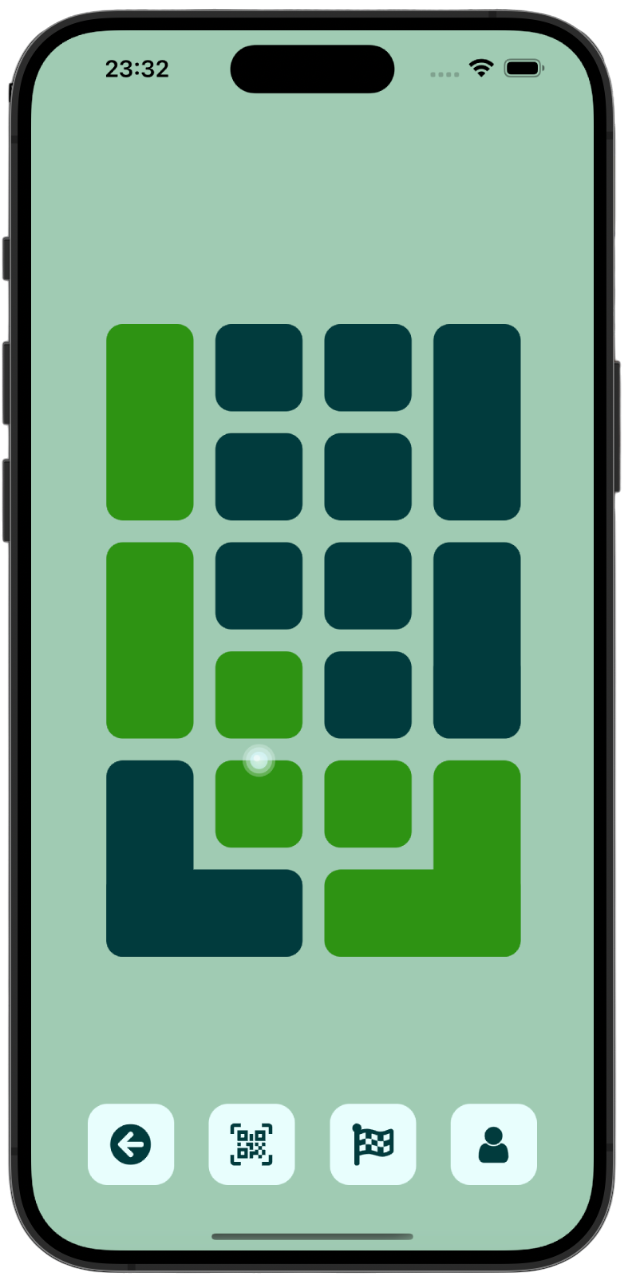
\includegraphics[width=0.3\textwidth]{images/front/navigation_moved.png}
\end{center}

\subsubsection{Profil użytkownika}

Ekran użytkownika umożliwia interakcję z chatbotem oraz zarządzanie kontem użytkownika, w tym możliwość wylogowania się z aplikacji.

\begin{center}
    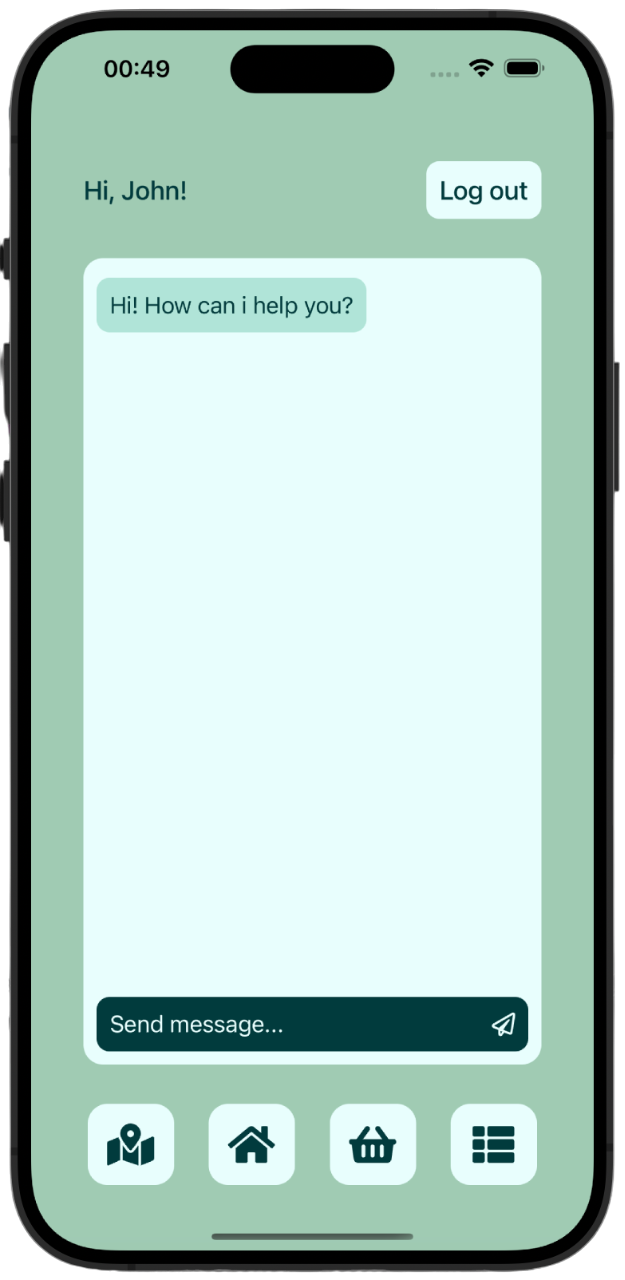
\includegraphics[width=0.3\textwidth]{images/front/user_page.png}
\end{center}

Na górze ekranu znajduje się powitanie użytkownika, wyświetlające jego imię, które jest pobierane z lokalnej pamięci aplikacji, aktualizowanej podczas poprawnego logowania. Obok powitania znajduje się przycisk \textit{Log out}, umożliwiający wylogowanie się z aplikacji i przekierowanie użytkownika na stronę główną. Wraz z kliknięciem tego przycisku czyszczona jest pamięć podręczna aplikacji, co skutkuje przerwaniem sesji i koniecznością ponownego zalogowania.

Główną część ekranu zajmuje chatbot, który pozwala na interakcję z użytkownikiem. Działa on w identyczny sposób, co wspomniany we wcześniejszych sekcjach dymek chatu, stąd zostanie on omówiony w osobnym rozdziale.

Dolną część ekranu zajmuje pasek nawigacyjny, który umożliwia przejście do innych sekcji aplikacji. Należą do nich: mapa sklepów, kategorie produktów, koszyk oraz strona tytułowa.


\subsection{Szczegółowe omówienie implementacji}
\subsubsection{Strona tytułowa}


\section{Serwer aplikacji}
Serwer jest odpowiedzialny za przetwarzanie żądań użytkownika, a także za komunikację z bazą danych. Został zaimplementowany w języku JavaScript przy użyciu platformy Node.js oraz struktury (ang. \textit{framework}) Express.js. Node.js pozwala na uruchamianie JavaScript po stronie serwera, co umożliwia tworzenie wydajnych i skalowalnych aplikacji. Express.js, będący minimalistycznym frameworkiem działającym na Node.js, upraszcza proces budowy aplikacji internetowych. Serwer nasłuchuje na zapytania HTTP, przetwarza je i zwraca odpowiedź, a do komunikacji z bazą danych PostgreSQL wykorzystuje odpowiednie moduły Node.js.


\subsection{JavaScript}
JavaScript jest podstawowym językiem programowania w sieci Web. Zdecydowana większość współczesnych stron internetowych wykorzystuje JavaScript, a wszystkie nowoczesne przeglądarki internetowe — zarówno na komputerach stacjonarnych, konsolach do gier, tabletach, jak i smartfonach — posiadają wbudowane interpretery tego języka. Dzięki temu JavaScript stał się najbardziej wszechobecnym językiem programowania w historii. Wraz z HTML, odpowiadającym za treść stron, oraz CSS, definiującym ich wygląd, JavaScript stanowi podstawowy zestaw technologii, które każdy programista webowy musi opanować, aby określać zachowanie stron internetowych. \cite{flanagan2011javascript}


\subsection{Node.js}
Node.js umożliwia programistom wykorzystywanie JavaScript po stronie serwera, co pozwala na tworzenie aplikacji full-stack przy użyciu jednego języka. Dzięki architekturze wspierającej asynchroniczne i nieblokujące operacje I/O świetnie sprawdza się w obsłudze wielu jednoczesnych połączeń. \cite{peters2017building}

Dzięki architekturze opartej na zdarzeniach oraz jednowątkowemu modelowi działania, Node.js idealnie nadaje się do tworzenia aplikacji czasu rzeczywistego, takich jak czaty, narzędzia do współpracy czy usługi streamingowe. \cite{peters2017building}

\subsection{Express.js}
Express.js to minimalistyczny framework dla Node.js, który pozwala na szybkie tworzenie aplikacji internetowych. Dzięki swojej prostocie i elastyczności jest jednym z najpopularniejszych frameworków dla Node.js.

Framework Express.js umożliwia dynamiczny routing, pozwalając programistom na definiowanie wzorców URL i przypisywanie ich do określonej logiki aplikacji. Taka elastyczność ułatwia zarządzanie złożonymi strukturami aplikacji poprzez wiązanie punktów końcowych z odpowiednimi kontrolerami. \cite{peters2017building}
